\chapter{Validierung}
\label{cha:Validierung}

In diesem Kapitel testen wir die Lernfähigkeit und die Lerndauer des TD-Q Agenten, in der Strategiespielumgebungen 9 Spielfelder Tic Tac Toe und 16 Spielfelder Tic Tac Toe. Wir testen ebenso die Spielstärke des (nicht lernenden) vorausschauenden Tic Tac Toe Heuristik Agenten. Der lernende und der nicht lernende Agent spielen genau 100 Testspiele gegeneinander und gegen einen Zufallsagenten. \\

Der TD-Q Agent wird 3 verschiedenen Lernphasen ausführen. Die Lernphasen unterscheiden sich in der Anzahl der Trainingsspiele. Untersucht werden vom TD-Q Agenten gelernte Strategien, die in 100 Trainingsspielen (Lernphase 1), in 1.000 Trainingsspielen (Lernphase 2) und in 10.000 Trainingsspielen, gegen sich selbst, trainiert wurden. Jede dieser Lernphasen wird für das 9 Spielfelder Tic Tac Toe und das 16 Spielfelder Tic Tac Toe ausgeführt. \\

Im nächsten Kapitel \ref{cha:Auswertung} werden wir erklären warum wir den TD-Q Lernenden Agenten keine Strategie für Reversi lernen lassen. Die Ergebnisse der Tests für das 9 Spielfelder Tic Tac Toe und das 16 Spielfelder Tic Tac Toe werden diese Erklärung belegen. \\

Die für das Testen der Agenten implementierten Strategiespielumgebungen wurden mit dem Python Paket ''unittest'' getestet. Die Tests der Tic Tac Toe Strategiespielumgebung befinden sich in der Datei ''TestTicTacToe.py'' und die Tests der Reversi Strategiespielumgebung befinden sich in der Datei ''TestReversi.py''. In diesen sind die wichtigsten Funktionalitäten der Strategiespielumgebungen ausgeführt und mit ''asserts'' getestet. Alle Tests der Strategiespielumgebungen waren positiv und könnten bei bedarf wiederholt werden. \\

\section{Tic Tac Toe - 9 Spielfelder}
In diesem Abschnitt testen wir den vorausschauenden Heuristik Agenten und den TD-Q Agenten gegen einen Zufallsagenten und gegeneinander, in einem 9 Spielfelder Tic Tac Toe. 

\subsection{Heuristik gegen Zufall}
Der vorausschauende Heuristik Agent gewinnt mit einer 64\% Gewinnquote, wenn der Zufallsagent beginnt und mit einer 83\% Gewinnquote, wenn er selbst beginnt.

\myparagraph{Der Zufallsagent beginnt:}
Der vorausschauende Heuristik Agent gewinnt 64 Testspiele, der Zufallsagent gewinnt 4 Testspiele und es werden 32 unentschieden erspielt.

\myparagraph{Der Heuristik Agent beginnt:}
Der vorausschauende Heuristik Agent gewinnt 83 Testspiele, der Zufallsagent gewinnt 3 Testspiele und es werden 14 unentschieden erspielt. 

\subsection{TD-Q Lernen in 100 Trainingsspielen}
\begin{itemize}
\item Lernzeit: ungefähr 5 Minuten

\item Siege gegen den beginnenden Zufallsagenten: 37
\item Niederlagen gegen den beginnenden Zufallsagenten: 59

\item Siege gegen den nachziehenden Zufallsagenten: 73
\item Niederlagen gegen den nachziehenden Zufallsagenten: 16

\item Siege gegen den beginnenden Heuristik Agenten: 0
\item Niederlagen gegen den beginnenden Heuristik Agenten: 100

\item Siege gegen den nachziehenden Heuristik Agenten: 0
\item Niederlagen gegen den nachziehenden Heuristik Agenten: 100
\end{itemize}

\subsection{TD-Q Lernen in 1.000 Trainingsspielen}
\begin{itemize}
\item Lernzeit: ungefähr 30 Minuten

\item Siege gegen den beginnenden Zufallsagenten: 41
\item Niederlagen gegen den beginnenden Zufallsagenten: 44

\item Siege gegen den nachziehenden Zufallsagenten: 79
\item Niederlagen gegen den nachziehenden Zufallsagenten: 15

\item Siege gegen den beginnenden Heuristik Agenten: 0
\item Niederlagen gegen den beginnenden Heuristik Agenten: 100

\item Siege gegen den nachziehenden Heuristik Agenten: 0
\item Niederlagen gegen den nachziehenden Heuristik Agenten: 0

\end{itemize}


\subsection{TD-Q Lernen in 10.000 Trainingsspielen}
\begin{itemize}
\item Lernzeit: ungefähr 180 Minuten

\item Siege gegen den beginnenden Zufallsagenten: 49
\item Niederlagen gegen den beginnenden Zufallsagenten: 38

\item Siege gegen den nachziehenden Zufallsagenten: 92
\item Niederlagen gegen den nachziehenden Zufallsagenten: 8

\item Siege gegen den beginnenden Heuristik Agenten: 0
\item Niederlagen gegen den beginnenden Heuristik Agenten: 100 

\item Siege gegen den nachziehenden Heuristik Agenten: 0
\item Niederlagen gegen den nachziehenden Heuristik Agenten: 100 
\end{itemize}
\newpage

\section{Tic Tac Toe - 16 Spielfelder}
In diesem Abschnitt testen wir den vorausschauenden Heuristik Agenten und den TD-Q Agenten gegen einen Zufallsagenten und gegeneinander, in einem 16 Spielfelder Tic Tac Toe. 

\subsection{Heuristik gegen Zufall}
Der vorausschauende Heuristik Agent gewinnt mit einer 88\% Gewinnquote, wenn der Zufallsagent beginnt und mit einer 100\% Gewinnquote, wenn er selbst beginnt.

\myparagraph{Der Zufallsagent beginnt:}
Der vorausschauende Heuristik Agent gewinnt 88 Testspiele, der Zufallsagent gewinnt 0 Testspiele und es werden 12 unentschieden erspielt.

\myparagraph{Der Heuristik Agent beginnt:}
Der vorausschauende Heuristik Agent gewinnt 100 Testspiele, der Zufallsagent gewinnt 0 Testspiele und es werden 0 unentschieden erspielt.

\subsection{TD-Q Lernen in 100 Trainingsspielen}
\begin{itemize}
\item Lernzeit: ungefähr 25 Minuten

\item Siege gegen den beginnenden Zufallsagenten: 52
\item Niederlagen gegen den beginnenden Zufallsagenten: 22 

\item Siege gegen den nachziehenden Zufallsagenten: 51
\item Niederlagen gegen den nachziehenden Zufallsagenten: 42 

\item Siege gegen den beginnenden Heuristik Agenten: 0
\item Niederlagen gegen den beginnenden Heuristik Agenten: 100

\item Siege gegen den nachziehenden Heuristik Agenten: 0
\item Niederlagen gegen den nachziehenden Heuristik Agenten: 100
\end{itemize}

\subsection{TD-Q Lernen in 1.000 Trainingsspielen}
\begin{itemize}
\item Lernzeit: ungefähr 180 Minuten

\item Siege gegen den beginnenden Zufallsagenten: 60
\item Niederlagen gegen den beginnenden Zufallsagenten: 23 

\item Siege gegen den nachziehenden Zufallsagenten: 48
\item Niederlagen gegen den nachziehenden Zufallsagenten: 34 

\item Siege gegen den beginnenden Heuristik Agenten: 0
\item Niederlagen gegen den beginnenden Heuristik Agenten: 100

\item Siege gegen den nachziehenden Heuristik Agenten: 0
\item Niederlagen gegen den nachziehenden Heuristik Agenten: 0

\end{itemize}


\subsection{TD-Q Lernen in 10.000 Trainingsspielen}
\begin{itemize}
\item Lernzeit: ungefähr 1440 Minuten

\item Siege gegen den beginnenden Zufallsagenten: 49
\item Niederlagen gegen den beginnenden Zufallsagenten: 32 

\item Siege gegen den nachziehenden Zufallsagenten: 57
\item Niederlagen gegen den nachziehenden Zufallsagenten: 18 

\item Siege gegen den beginnenden Heuristik Agenten: 0
\item Niederlagen gegen den beginnenden Heuristik Agenten: 100 

\item Siege gegen den nachziehenden Heuristik Agenten: 0
\item Niederlagen gegen den nachziehenden Heuristik Agenten: 100 
\end{itemize}

\begin{figure}[!htbp]
  \centering
  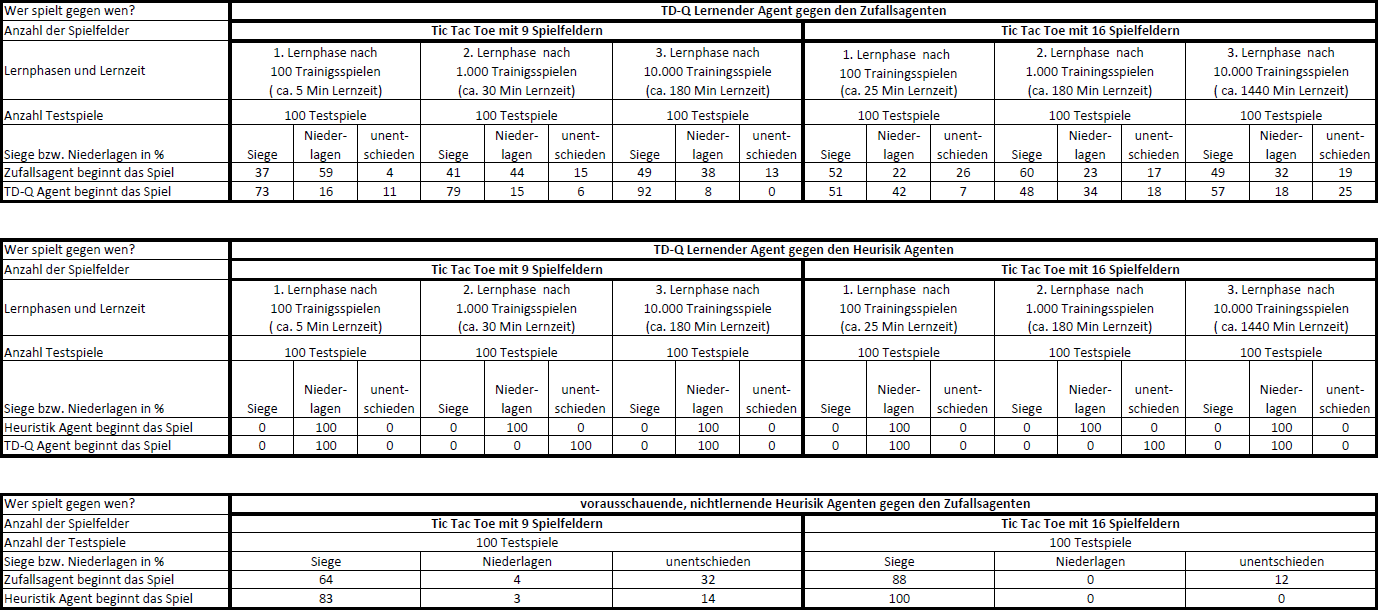
\includegraphics[angle = 90, scale = 0.8]{inhalt/abbildungen/testergebnisse.png}
  \caption{Die Ergebnisse der Agententests.}
  \label{fig:Ergebnisse der Agententests}
\end{figure} 